\part{Classic Variants and Improvements}

\chapter{Classic Variants of GAN}
Generative Adversarial Networks (GANs) have seen numerous improvements and adaptations since their introduction. Among these variations, Conditional GANs (CGANs)~\cite{mirza2014conditional} have gained significant attention for their ability to incorporate additional information during the generation process, allowing more control over the output~\cite{wang2018cgan}. In this chapter, we will explore CGANs in detail, discussing their fundamental concepts and their applications, especially in image generation tasks.

\section{Conditional Generative Adversarial Networks (CGAN)}
Conditional GANs (CGANs) extend the original GAN framework by conditioning the generation process on some external information~\cite{li2020gan}. This allows the generator to not only generate random samples but to generate samples based on specific input conditions. This conditioning can be any type of information, such as class labels or image attributes~\cite{mirza2014conditional, wang2018cgan}.

\subsection{Basic Concept of Conditional GAN}
In a traditional GAN, the generator produces output solely based on random noise. In a CGAN, however, the generator and discriminator both receive an additional input: a condition. This condition can be any type of auxiliary information, such as a class label in a supervised learning problem or some attribute of the data~\cite{wang2018cgan}. The key idea is that this condition is incorporated into both the generator and discriminator to influence the data generation process.

Formally, the CGAN objective can be written as:

\[
\min_G \max_D \mathbb{E}_{x \sim p_{\text{data}}(x)}[\log D(x|y)] + \mathbb{E}_{z \sim p_z(z)}[\log(1 - D(G(z|y)))]
\]

Where:
\begin{itemize}
    \item \( G(z|y) \): The generator that produces data based on random noise \( z \) and a condition \( y \).
    \item \( D(x|y) \): The discriminator that classifies whether a given data sample \( x \) is real or fake, conditioned on \( y \).
    \item \( y \): The conditional input, such as a label or feature.
\end{itemize}

The generator aims to produce samples that not only look real but also match the given condition \( y \), while the discriminator tries to distinguish between real and generated data while also considering the condition~\cite{wang2018cgan, devries2019evaluation}.

\subsection{Illustrative Example of Conditional GAN}
To better understand the concept, let's consider an example where we want to generate images of handwritten digits from the MNIST dataset~\cite{deng2012mnist}, but with the ability to control which digit the generator should produce (i.e., we want to generate a specific digit like 3 or 7)~\cite{thekumparampil2018robustness}.

\begin{figure}[htbp]
    \centering
    \includegraphics[width=0.8\textwidth]{figs/cgan.pdf}
    \caption{The basic architecture of a Conditional GAN (CGAN).}
\end{figure}

In this case, the condition \( y \) is the label of the digit (0 through 9), and the generator will learn to produce an image of the specified digit based on both the random noise \( z \) and the label \( y \). The discriminator will evaluate not only whether the image looks real, but also whether the generated image corresponds to the specified label.

\subsection{How Conditioning Works in CGAN}
In a CGAN, the condition \( y \) can be concatenated with the input noise vector \( z \) and fed into the generator. Similarly, the discriminator takes both the condition \( y \) and the generated or real data as input. This can be done by either concatenating \( y \) with the input or by using other more sophisticated mechanisms such as embedding layers~\cite{mirza2014conditional}.

Let's break this down in Python using PyTorch.

\subsection{Step-by-Step Example of CGAN}
We will implement a Conditional GAN for generating MNIST digits conditioned on the digit labels. First, we will set up the required libraries:

\begin{lstlisting}[style=cmd]
pip install torch torchvision matplotlib
\end{lstlisting}

Now, let's implement the CGAN architecture using PyTorch.

\subsubsection{Step 1: Import Necessary Libraries}
We will start by importing the necessary libraries and setting up some basic parameters.

\begin{lstlisting}[style=python]
import torch
import torch.nn as nn
import torch.optim as optim
import torchvision
import torchvision.transforms as transforms
import matplotlib.pyplot as plt

# Hyperparameters
latent_dim = 100  # Dimension of the noise vector
num_classes = 10  # Number of digit classes in MNIST
image_size = 28   # Image dimensions (28x28 for MNIST)
batch_size = 64
lr = 0.0002
epochs = 50
\end{lstlisting}

\subsubsection{Step 2: Define the Generator and Discriminator}
We need to modify the generator and discriminator to accept both the noise vector \( z \) and the conditional label \( y \). One common approach is to concatenate \( z \) with a one-hot encoded label vector for \( y \).

\begin{lstlisting}[style=python]
# Generator model
class Generator(nn.Module):
    def __init__(self, latent_dim, num_classes, img_size):
        super(Generator, self).__init__()
        self.label_emb = nn.Embedding(num_classes, num_classes)
        self.model = nn.Sequential(
            nn.Linear(latent_dim + num_classes, 128),
            nn.ReLU(),
            nn.Linear(128, 256),
            nn.BatchNorm1d(256, 0.8),
            nn.ReLU(),
            nn.Linear(256, 512),
            nn.BatchNorm1d(512, 0.8),
            nn.ReLU(),
            nn.Linear(512, img_size * img_size),
            nn.Tanh()
        )
    
    def forward(self, noise, labels):
        # Concatenate noise and label embeddings
        gen_input = torch.cat((noise, self.label_emb(labels)), -1)
        img = self.model(gen_input)
        img = img.view(img.size(0), 1, image_size, image_size)
        return img

# Discriminator model
class Discriminator(nn.Module):
    def __init__(self, num_classes, img_size):
        super(Discriminator, self).__init__()
        self.label_emb = nn.Embedding(num_classes, num_classes)
        self.model = nn.Sequential(
            nn.Linear(num_classes + img_size * img_size, 512),
            nn.LeakyReLU(0.2, inplace=True),
            nn.Linear(512, 256),
            nn.LeakyReLU(0.2, inplace=True),
            nn.Linear(256, 1),
            nn.Sigmoid()
        )

    def forward(self, img, labels):
        # Flatten image and concatenate with label embeddings
        img_flat = img.view(img.size(0), -1)
        d_in = torch.cat((img_flat, self.label_emb(labels)), -1)
        validity = self.model(d_in)
        return validity
\end{lstlisting}

In the generator, we take the noise \( z \) and the label \( y \) as inputs and concatenate them before feeding them into the network. Similarly, in the discriminator, we flatten the image and concatenate it with the label embedding.

\subsubsection{Step 3: Training the CGAN}
Next, we set up the loss function and optimizers, and then train the CGAN.

\begin{lstlisting}[style=python]
# Loss function
adversarial_loss = nn.BCELoss()

# Initialize generator and discriminator
generator = Generator(latent_dim, num_classes, image_size)
discriminator = Discriminator(num_classes, image_size)

# Optimizers
optimizer_g = optim.Adam(generator.parameters(), lr=lr, betas=(0.5, 0.999))
optimizer_d = optim.Adam(discriminator.parameters(), lr=lr, betas=(0.5, 0.999))

# Load MNIST dataset
transform = transforms.Compose([transforms.ToTensor(), transforms.Normalize([0.5], [0.5])])
dataloader = torch.utils.data.DataLoader(
    torchvision.datasets.MNIST('./data', train=True, download=True, transform=transform),
    batch_size=batch_size, shuffle=True
)

# Training loop
for epoch in range(epochs):
    for i, (imgs, labels) in enumerate(dataloader):
        
        # Adversarial ground truths
        valid = torch.ones(imgs.size(0), 1)
        fake = torch.zeros(imgs.size(0), 1)

        # Configure input
        real_imgs = imgs
        labels = labels

        # ---------------------
        #  Train Discriminator
        # ---------------------
        optimizer_d.zero_grad()

        # Sample noise and labels as generator input
        z = torch.randn(imgs.size(0), latent_dim)
        gen_labels = torch.randint(0, num_classes, (imgs.size(0),))

        # Generate a batch of images
        gen_imgs = generator(z, gen_labels)

        # Loss for real images
        real_loss = adversarial_loss(discriminator(real_imgs, labels), valid)
        # Loss for fake images
        fake_loss = adversarial_loss(discriminator(gen_imgs.detach(), gen_labels), fake)
        # Total discriminator loss
        d_loss = (real_loss + fake_loss) / 2

        d_loss.backward()
        optimizer_d.step()

        # -----------------
        #  Train Generator
        # -----------------
        optimizer_g.zero_grad()

        # Loss for generator
        g_loss = adversarial_loss(discriminator(gen_imgs, gen_labels), valid)

        g_loss.backward()
        optimizer_g.step()

        print(f"[Epoch {epoch}/{epochs}] [Batch {i}/{len(dataloader)}] [D loss: {d_loss.item():.4f}] [G loss: {g_loss.item():.4f}]")
\end{lstlisting}

In this training loop, the generator learns to produce MNIST digits conditioned on the class labels, while the discriminator learns to classify whether an image is real or generated, based on both the image and its corresponding label.

\section{Application of CGAN in Image Generation}
Conditional GANs are widely used in various tasks that require controlled data generation~\cite{mirza2014conditional, wang2018cgan, devries2019evaluation}. One of the most common applications is in image generation tasks~\cite{bao2017cvae, liu2019multi}, where CGANs allow users to generate specific types of images based on certain conditions.

\subsection{Example: Handwritten Digit Generation}
As seen in the above implementation, CGAN can be used to generate handwritten digits conditioned on the label of the digit~\cite{liu2019multi}. This means that we can specify which digit (from 0 to 9) we want the generator to create, providing more control over the output compared to a standard GAN.

\subsection{Image-to-Image Translation}
Another popular application of CGANs is in image-to-image translation~\cite{yi2017dualgan}, where the goal is to generate a target image based on an input image. For example:
\begin{itemize}
    \item Generating a colored image from a grayscale image.
    \item Translating a daytime image to a nighttime image.
    \item Converting a sketch to a photorealistic image.
\end{itemize}
In such tasks, the condition \( y \) is often the input image, and the generator learns to translate the input into a desired output based on the condition.

\section{Summary}
In this chapter, we explored the concept of Conditional GANs (CGANs), which extend the original GAN framework by conditioning the generation process on additional information such as labels or attributes. CGANs allow for more control over the generated output and have been successfully applied to various tasks, including digit generation~\cite{liu2019multi} and image-to-image translation~\cite{yi2017dualgan}. Through a detailed PyTorch implementation, we demonstrated how to build and train a CGAN, offering a practical example for beginners to better understand how CGANs function.










\section{Deep Convolutional Generative Adversarial Networks (DCGAN)}
Deep Convolutional Generative Adversarial Networks (DCGAN)~\cite{radford2015unsupervised} are a variant of GANs where convolutional neural networks (CNNs) are used instead of fully connected layers~\cite{luo2021case}, especially in the Generator and Discriminator. This architectural change allows DCGANs to leverage the spatial hierarchical nature of images, making them particularly powerful for image generation tasks. 

\subsection{The Role of Convolutional Networks in GANs}
Convolutional neural networks (CNNs)~\cite{lecun2015deep} are specifically designed to work with grid-like data, such as images. Unlike fully connected layers, where each neuron is connected to all neurons in the previous layer, convolutional layers~\cite{radford2015unsupervised} use filters (also called kernels) to perform localized operations over small patches of the image~\cite{lecun2015deep, o2015cnn}. This process captures spatial dependencies, such as edges or textures, that are essential for image understanding and generation.

In the context of GANs, using CNNs allows the Generator to produce images with better quality and sharper details~\cite{goodfellow2014generative, radford2015unsupervised}. Similarly, the Discriminator can use convolutional layers to more effectively distinguish between real and generated images, recognizing subtle differences in structure and texture.

\textbf{Example of a Convolutional Layer in PyTorch:}

\begin{lstlisting}[style=python]
import torch
import torch.nn as nn

# Example of a simple convolutional layer in PyTorch
conv_layer = nn.Conv2d(in_channels=3, out_channels=64, kernel_size=4, stride=2, padding=1)

# Input image: 3 channels (RGB), size 64x64
input_image = torch.randn(1, 3, 64, 64)

# Apply convolution
output = conv_layer(input_image)
print(output.shape)  # Output will have 64 channels, reduced spatial dimensions
\end{lstlisting}

In this example, the convolutional layer takes a 64x64 RGB image as input and applies 64 filters with a kernel size of 4x4. The stride of 2 reduces the spatial dimensions, while padding ensures the output image size is manageable. This operation helps extract important features such as edges, corners, and textures.

\subsection{DCGAN Architecture and Implementation}
The DCGAN architecture introduces several modifications compared to standard GANs:

\begin{itemize}
    \item \textbf{No fully connected layers}: Both the Generator and Discriminator avoid using fully connected layers in favor of convolutional layers. This helps the networks scale better with image size and capture local patterns effectively~\cite{radford2015unsupervised}.
    \item \textbf{Batch normalization}: Batch normalization is used after most layers to stabilize training by normalizing the activations, which allows for faster convergence.
    \item \textbf{Leaky ReLU}: In the Discriminator, the Leaky ReLU~\cite{dubey2019comparative} activation function is used, which allows a small gradient when the activation is negative, addressing the problem of dying ReLUs.
    \item \textbf{Transposed convolutions}: In the Generator, transposed convolutions~\cite{jansson2012deconvolution} (also known as deconvolutions) are used to upsample noise into an image.
\end{itemize}

\textbf{DCGAN Generator and Discriminator in PyTorch:}

\begin{lstlisting}[style=python]
# DCGAN Generator
class DCGAN_Generator(nn.Module):
    def __init__(self, noise_dim):
        super(DCGAN_Generator, self).__init__()
        self.model = nn.Sequential(
            nn.ConvTranspose2d(noise_dim, 512, 4, 1, 0),  # First layer, fully connected equivalent
            nn.BatchNorm2d(512),
            nn.ReLU(True),
            nn.ConvTranspose2d(512, 256, 4, 2, 1),  # Upsample to 8x8
            nn.BatchNorm2d(256),
            nn.ReLU(True),
            nn.ConvTranspose2d(256, 128, 4, 2, 1),  # Upsample to 16x16
            nn.BatchNorm2d(128),
            nn.ReLU(True),
            nn.ConvTranspose2d(128, 64, 4, 2, 1),  # Upsample to 32x32
            nn.BatchNorm2d(64),
            nn.ReLU(True),
            nn.ConvTranspose2d(64, 3, 4, 2, 1),    # Upsample to 64x64 (RGB)
            nn.Tanh()  # Tanh activation for output images
        )

    def forward(self, x):
        return self.model(x)

# DCGAN Discriminator
class DCGAN_Discriminator(nn.Module):
    def __init__(self):
        super(DCGAN_Discriminator, self).__init__()
        self.model = nn.Sequential(
            nn.Conv2d(3, 64, 4, 2, 1),   # Downsample to 32x32
            nn.LeakyReLU(0.2, inplace=True),
            nn.Conv2d(64, 128, 4, 2, 1), # Downsample to 16x16
            nn.BatchNorm2d(128),
            nn.LeakyReLU(0.2, inplace=True),
            nn.Conv2d(128, 256, 4, 2, 1),# Downsample to 8x8
            nn.BatchNorm2d(256),
            nn.LeakyReLU(0.2, inplace=True),
            nn.Conv2d(256, 512, 4, 2, 1),# Downsample to 4x4
            nn.BatchNorm2d(512),
            nn.LeakyReLU(0.2, inplace=True),
            nn.Conv2d(512, 1, 4, 1, 0),  # Output a single scalar value (real or fake)
            nn.Sigmoid()                 # Sigmoid activation for binary classification
        )

    def forward(self, x):
        return self.model(x)

# Example usage:
noise = torch.randn(1, 100, 1, 1)  # Random noise for Generator
gen = DCGAN_Generator(100)
disc = DCGAN_Discriminator()

generated_image = gen(noise)
disc_output = disc(generated_image)

print(generated_image.shape)  # Should output: torch.Size([1, 3, 64, 64])
print(disc_output.shape)      # Should output: torch.Size([1, 1, 1, 1])
\end{lstlisting}

In this example, the Generator starts with noise of shape \(100 \times 1 \times 1\), which is upsampled through a series of transposed convolutions to a \(64 \times 64\) RGB image. The Discriminator takes this image and progressively downsamples it through convolutions~\cite{lecun2015deep}, outputting a single value indicating whether the image is real or fake.

\section{Information Maximizing Generative Adversarial Networks (InfoGAN)}
InfoGAN~\cite{chen2016infogan} is an extension of GANs that introduces an information-theoretic objective to maximize mutual information between a subset of latent variables and the generated data. This enables InfoGAN to learn interpretable and disentangled representations in an unsupervised manner~\cite{kurutach2018learning}, making it highly useful for understanding the structure of the data without requiring labeled examples.

\subsection{Introducing the Information Maximization Objective}
The key innovation in InfoGAN is the addition of a new objective to maximize the mutual information between the latent code \(c\) and the generated data \(G(z, c)\). In a standard GAN, the latent vector \(z\) is random noise, and the generated data is not necessarily interpretable. However, in InfoGAN, we split \(z\) into two parts:

\begin{itemize}
    \item \textbf{Random noise} \(z\), which is the standard noise vector used by GANs.
    \item \textbf{Latent code} \(c\), which encodes specific information that we want the Generator to learn.
\end{itemize}

Maximizing the mutual information \(I(c; G(z, c))\) encourages the Generator to produce data that reflects the information encoded in \(c\). This gives us control over certain aspects of the generated data, such as the orientation of a digit in an image or its style, while still operating in an unsupervised learning setting~\cite{chen2016infogan}.

The InfoGAN architecture introduces a separate network called the \textbf{Q-network}, which approximates the posterior distribution of the latent code \(c\) given the generated data. This allows InfoGAN to compute and maximize the mutual information efficiently.

\subsubsection{Example: InfoGAN Latent Code Control}
Let's assume we are generating images of handwritten digits using InfoGAN. The latent code \(c\) might encode the following information:

\begin{itemize}
    \item \(c_1\): The digit's thickness.
    \item \(c_2\): The digit's rotation angle.
    \item \(c_3\): The digit's style.
\end{itemize}

By controlling the values of \(c_1\), \(c_2\), and \(c_3\), we can generate images with specific thickness, rotation, or style, even though the model was trained without labeled data.

\textbf{InfoGAN Training in PyTorch:}

\begin{lstlisting}[style=python]
# InfoGAN with additional latent code c
class InfoGAN_Generator(nn.Module):
    def __init__(self, noise_dim, code_dim):
        super(InfoGAN_Generator, self).__init__()
        self.model = nn.Sequential(
            nn.ConvTranspose2d(noise_dim + code_dim, 512, 4, 1, 0),
            nn.BatchNorm2d(512),
            nn.ReLU(True),
            nn.ConvTranspose2d(512, 256, 4, 2, 1),
            nn.BatchNorm2d(256),
            nn.ReLU(True),
            nn.ConvTranspose2d(256, 128, 4, 2, 1),
            nn.BatchNorm2d(128),
            nn.ReLU(True),
            nn.ConvTranspose2d(128, 64, 4, 2, 1),
            nn.BatchNorm2d(64),
            nn.ReLU(True),
            nn.ConvTranspose2d(64, 3, 4, 2, 1),
            nn.Tanh()
        )

    def forward(self, noise, code):
        x = torch.cat([noise, code], dim=1)  # Concatenate noise and code
        return self.model(x)

# Q-network to approximate posterior q(c|x)
class InfoGAN_Q_Network(nn.Module):
    def __init__(self):
        super(InfoGAN_Q_Network, self).__init__()
        self.model = nn.Sequential(
            nn.Conv2d(3, 64, 4, 2, 1),
            nn.LeakyReLU(0.2, inplace=True),
            nn.Conv2d(64, 128, 4, 2, 1),
            nn.BatchNorm2d(128),
            nn.LeakyReLU(0.2, inplace=True),
            nn.Conv2d(128, 256, 4, 2, 1),
            nn.BatchNorm2d(256),
            nn.LeakyReLU(0.2, inplace=True),
            nn.Conv2d(256, 512, 4, 2, 1),
            nn.BatchNorm2d(512),
            nn.LeakyReLU(0.2, inplace=True),
            nn.Flatten(),
            nn.Linear(512 * 4 * 4, 128),
            nn.ReLU(True),
            nn.Linear(128, 10)  # Assume latent code c is 10-dimensional
        )

    def forward(self, x):
        return self.model(x)

# Example usage:
noise = torch.randn(1, 100, 1, 1)  # Random noise
code = torch.randn(1, 10, 1, 1)    # Latent code

gen = InfoGAN_Generator(100, 10)
q_net = InfoGAN_Q_Network()

generated_image = gen(noise, code)
q_output = q_net(generated_image)

print(generated_image.shape)  # Should output: torch.Size([1, 3, 64, 64])
print(q_output.shape)         # Should output: torch.Size([1, 10])
\end{lstlisting}

In this example, the Generator takes both noise and a latent code as input, producing an image that is influenced by the code. The Q-network tries to estimate the latent code from the generated image, allowing the model to learn how the latent code affects the generated data.

\subsection{InfoGAN in Unsupervised Learning}
One of the key advantages of InfoGAN is its ability to learn interpretable features in an unsupervised setting. In many real-world scenarios, labeled data is scarce or expensive to obtain, so having a model that can automatically discover and disentangle important features without supervision is highly valuable.

In InfoGAN, the latent code \(c\) provides a mechanism for this unsupervised learning. By maximizing the mutual information between the latent code and the generated data, InfoGAN encourages the Generator to create data that reflects the structure of the input code. This allows InfoGAN to discover meaningful and disentangled representations of the data, such as variations in object shape, color, or orientation, without needing explicit labels~\cite{mugunthan2021dpd}.

\textbf{Example: Unsupervised Learning of Handwritten Digits}

Consider a dataset of handwritten digits (e.g., MNIST). InfoGAN can learn to control different aspects of the digits, such as:

\begin{itemize}
    \item The digit's thickness (controlled by \(c_1\)).
    \item The rotation angle (controlled by \(c_2\)).
    \item The style or stroke (controlled by \(c_3\)).
\end{itemize}

Even though the model is trained without knowing these specific features, InfoGAN learns to disentangle them naturally~\cite{chen2016infogan}. By manipulating the latent code during generation, we can generate digits with specific characteristics, gaining insight into the structure of the data in an unsupervised manner.










\section{Laplacian Pyramid GAN (LAPGAN)}
Understanding LAPGAN~\cite{denton2015deep} is crucial for generating high-resolution images with fine details. In this section, we will delve into the hierarchical generation process~\cite{jin2020hierarchical} of LAPGAN and explore its applications in image detail generation.

\subsection{Hierarchical Generation Process}

The Laplacian Pyramid Generative Adversarial Network (LAPGAN) is a GAN architecture that generates images in a coarse-to-fine fashion using a pyramid of generators and discriminators. Instead of generating a high-resolution image in one pass, LAPGAN breaks down the image generation process into multiple stages, each responsible for generating images at different resolutions~\cite{jin2020hierarchical}.

\subsubsection{Laplacian Pyramid Concept}

The Laplacian Pyramid is a technique used in image processing to represent images at multiple scales or resolutions~\cite{zhang2018photographic}. It involves decomposing an image into a set of band-pass filtered images (Laplacian images) and a low-resolution residual image.

To construct a Laplacian Pyramid, we perform the following steps:

\begin{enumerate}
    \item \textbf{Gaussian Pyramid Construction}: Create a series of images where each subsequent image is a downsampled (usually by a factor of 2) version of the previous one using a Gaussian filter.
    \item \textbf{Laplacian Images Computation}: Subtract the upsampled version of each lower-resolution image from the current resolution image to obtain the Laplacian images.
\end{enumerate}

By reconstructing the original image from the Laplacian Pyramid, we can add back the details at each level, starting from the lowest resolution.

\subsubsection{LAPGAN Architecture}

In LAPGAN, the image generation process is divided into multiple levels corresponding to different resolutions. Each level consists of a generator and a discriminator:

\begin{itemize}
    \item \textbf{Generator at Level \( i \)}: Generates a high-resolution image \( x_i \) conditioned on the upsampled image \( x_{i-1}^{\uparrow} \) from the previous level and a random noise vector \( z_i \).
    \item \textbf{Discriminator at Level \( i \)}: Evaluates the authenticity of the generated image \( x_i \) against the real images at the same resolution.
\end{itemize}

The overall generation process can be summarized as:

\[
x_0 = G_0(z_0) \\
x_i = G_i(x_{i-1}^{\uparrow}, z_i), \quad \text{for } i = 1, 2, ..., N
\]

Where:
\begin{itemize}
    \item \( x_0 \) is the initial low-resolution image generated from noise.
    \item \( x_{i-1}^{\uparrow} \) is the upsampled image from the previous level.
    \item \( G_i \) is the generator at level \( i \).
    \item \( z_i \) is the noise vector injected at level \( i \).
\end{itemize}

This hierarchical approach allows the model to focus on adding details progressively, making it easier to generate high-resolution images with fine details~\cite{denton2015deep}.

\subsubsection{Implementation Example}

Let's implement a simplified version of LAPGAN using PyTorch. We'll use a three-level pyramid to generate images of size \( 64 \times 64 \).

\begin{lstlisting}[style=python]
import torch
import torch.nn as nn
import torch.optim as optim
import torch.nn.functional as F

# Define the Generator for level 0 (16x16)
class GeneratorLevel0(nn.Module):
    def __init__(self):
        super(GeneratorLevel0, self).__init__()
        self.main = nn.Sequential(
            nn.Linear(100, 128),
            nn.ReLU(),
            nn.Linear(128, 16*16*3),
            nn.Tanh()
        )
    
    def forward(self, z):
        output = self.main(z)
        output = output.view(-1, 3, 16, 16)
        return output

# Define the Generator for higher levels (32x32 and 64x64)
class GeneratorLevelN(nn.Module):
    def __init__(self, input_channels):
        super(GeneratorLevelN, self).__init__()
        self.main = nn.Sequential(
            nn.Conv2d(input_channels, 64, kernel_size=3, padding=1),
            nn.ReLU(),
            nn.Conv2d(64, 3, kernel_size=3, padding=1),
            nn.Tanh()
        )
    
    def forward(self, x, z):
        z = z.view(-1, 1, x.size(2), x.size(3))
        input = torch.cat([x, z], dim=1)
        output = self.main(input)
        return output

# Define the Discriminator for each level
class Discriminator(nn.Module):
    def __init__(self, image_size):
        super(Discriminator, self).__init__()
        self.main = nn.Sequential(
            nn.Conv2d(3, 64, kernel_size=4, stride=2),
            nn.LeakyReLU(0.2),
            nn.Conv2d(64, 128, kernel_size=4, stride=2),
            nn.LeakyReLU(0.2),
            nn.Flatten(),
            nn.Linear(128 * (image_size//4) * (image_size//4), 1),
            nn.Sigmoid()
        )
    
    def forward(self, x):
        return self.main(x)
\end{lstlisting}

In this example, we have:

\begin{itemize}
    \item \textbf{GeneratorLevel0}: Generates a \( 16 \times 16 \) image from a noise vector \( z \).
    \item \textbf{GeneratorLevelN}: Takes the upsampled image from the previous level, concatenated with a noise map, and outputs a higher-resolution image.
    \item \textbf{Discriminator}: Evaluates images at each resolution.
\end{itemize}

Next, we need to define the training process for each level.

\begin{lstlisting}[style=python]
# Instantiate generators and discriminators
G0 = GeneratorLevel0()
D0 = Discriminator(16)
G1 = GeneratorLevelN(4)  # 3 channels from upsampled image + 1 channel noise
D1 = Discriminator(32)
G2 = GeneratorLevelN(4)
D2 = Discriminator(64)

# Optimizers
optimizer_G0 = optim.Adam(G0.parameters(), lr=0.0002)
optimizer_D0 = optim.Adam(D0.parameters(), lr=0.0002)
optimizer_G1 = optim.Adam(G1.parameters(), lr=0.0002)
optimizer_D1 = optim.Adam(D1.parameters(), lr=0.0002)
optimizer_G2 = optim.Adam(G2.parameters(), lr=0.0002)
optimizer_D2 = optim.Adam(D2.parameters(), lr=0.0002)

# Loss function
criterion = nn.BCELoss()

# Training loop for each level
for epoch in range(num_epochs):
    ############################
    # Level 0 Training (16x16)
    ############################
    # Generate noise and fake images
    z0 = torch.randn(batch_size, 100)
    fake_images0 = G0(z0)
    
    # Get real images at 16x16 resolution
    real_images0 = get_real_images(16)
    
    # Train Discriminator D0
    optimizer_D0.zero_grad()
    # Real images
    outputs_real = D0(real_images0)
    labels_real = torch.ones(batch_size, 1)
    loss_D_real = criterion(outputs_real, labels_real)
    # Fake images
    outputs_fake = D0(fake_images0.detach())
    labels_fake = torch.zeros(batch_size, 1)
    loss_D_fake = criterion(outputs_fake, labels_fake)
    # Backprop and optimize
    loss_D0 = loss_D_real + loss_D_fake
    loss_D0.backward()
    optimizer_D0.step()
    
    # Train Generator G0
    optimizer_G0.zero_grad()
    outputs = D0(fake_images0)
    loss_G0 = criterion(outputs, labels_real)
    loss_G0.backward()
    optimizer_G0.step()
    
    ############################
    # Level 1 Training (32x32)
    ############################
    # Upsample images from Level 0
    upsampled_images0 = F.interpolate(fake_images0.detach(), scale_factor=2)
    # Generate noise map
    z1 = torch.randn(batch_size, 1, 32, 32)
    # Generate fake images at Level 1
    fake_images1 = G1(upsampled_images0, z1)
    
    # Get real images at 32x32 resolution
    real_images1 = get_real_images(32)
    
    # Train Discriminator D1
    optimizer_D1.zero_grad()
    # Real images
    outputs_real = D1(real_images1)
    labels_real = torch.ones(batch_size, 1)
    loss_D_real = criterion(outputs_real, labels_real)
    # Fake images
    outputs_fake = D1(fake_images1.detach())
    labels_fake = torch.zeros(batch_size, 1)
    loss_D_fake = criterion(outputs_fake, labels_fake)
    # Backprop and optimize
    loss_D1 = loss_D_real + loss_D_fake
    loss_D1.backward()
    optimizer_D1.step()
    
    # Train Generator G1
    optimizer_G1.zero_grad()
    outputs = D1(fake_images1)
    loss_G1 = criterion(outputs, labels_real)
    loss_G1.backward()
    optimizer_G1.step()
    
    ############################
    # Level 2 Training (64x64)
    ############################
    # Upsample images from Level 1
    upsampled_images1 = F.interpolate(fake_images1.detach(), scale_factor=2)
    # Generate noise map
    z2 = torch.randn(batch_size, 1, 64, 64)
    # Generate fake images at Level 2
    fake_images2 = G2(upsampled_images1, z2)
    
    # Get real images at 64x64 resolution
    real_images2 = get_real_images(64)
    
    # Train Discriminator D2
    optimizer_D2.zero_grad()
    # Real images
    outputs_real = D2(real_images2)
    labels_real = torch.ones(batch_size, 1)
    loss_D_real = criterion(outputs_real, labels_real)
    # Fake images
    outputs_fake = D2(fake_images2.detach())
    labels_fake = torch.zeros(batch_size, 1)
    loss_D_fake = criterion(outputs_fake, labels_fake)
    # Backprop and optimize
    loss_D2 = loss_D_real + loss_D_fake
    loss_D2.backward()
    optimizer_D2.step()
    
    # Train Generator G2
    optimizer_G2.zero_grad()
    outputs = D2(fake_images2)
    loss_G2 = criterion(outputs, labels_real)
    loss_G2.backward()
    optimizer_G2.step()
\end{lstlisting}

In this code:

\begin{itemize}
    \item We define separate generators and discriminators for each level.
    \item At each level, the generator takes the upsampled image from the previous level and a noise map to generate finer details.
    \item The discriminator at each level evaluates the generated images against real images at the same resolution.
    \item We use the Binary Cross-Entropy loss (\texttt{nn.BCELoss})~\cite{ruby2020binary} for training.
\end{itemize}

\subsection{Applications of LAPGAN in Image Detail Generation}

LAPGAN is particularly useful in generating high-resolution images with fine details, which is challenging for standard GAN architectures. By breaking down the generation process into hierarchical levels, LAPGAN can:

\begin{itemize}
    \item \textbf{Capture Global Structure}: The initial low-resolution generator focuses on generating the overall structure of the image~\cite{cao2015grarep}.
    \item \textbf{Add Fine Details}: Subsequent generators add details at increasingly finer scales, refining the image progressively.
    \item \textbf{Improve Training Stability}: Training smaller generators and discriminators at each level can be more stable and easier than training a single large network.
\end{itemize}

\subsubsection{Example: High-Resolution Face Generation}

Suppose we want to generate high-resolution images of faces at \( 256 \times 256 \) pixels. Using LAPGAN, we can divide the generation process into multiple levels:

\begin{enumerate}
    \item \textbf{Level 0}: Generate a coarse \( 64 \times 64 \) face image capturing the overall facial structure.
    \item \textbf{Level 1}: Refine to \( 128 \times 128 \) resolution, adding details like eyes, nose, and mouth shapes.
    \item \textbf{Level 2}: Finalize at \( 256 \times 256 \) resolution, adding skin textures, hair details, and other fine features.
\end{enumerate}

At each level, the generator focuses on adding the appropriate level of detail, conditioned on the upsampled image from the previous level~\cite{denton2015deep}.

\subsubsection{Benefits in Image Super-Resolution}

LAPGAN can also be applied to image super-resolution~\cite{lai2018fast} tasks, where the goal is to reconstruct high-resolution images from low-resolution inputs. By leveraging the hierarchical structure, LAPGAN can progressively upscale images while adding realistic details.

\subsubsection{Comparison with Other Methods}

Compared to traditional GANs, LAPGAN offers several advantages:

\begin{itemize}
    \item \textbf{Efficiency}: Training smaller networks at each level reduces computational requirements.
    \item \textbf{Quality}: Produces higher-quality images with better detail preservation.
    \item \textbf{Scalability}: Can be extended to generate very high-resolution images by adding more levels~\cite{lai2018fast}.
\end{itemize}

However, LAPGAN also has some limitations:

\begin{itemize}
    \item \textbf{Complexity}: The architecture is more complex due to multiple generators and discriminators~\cite{denton2015deep}.
    \item \textbf{Training Time}: Sequential training of multiple levels can increase the overall training time.
\end{itemize}

\subsection{Visualization of LAPGAN Architecture}

To better understand the structure of LAPGAN, consider the following diagram illustrating the hierarchical generation process:

\begin{center}
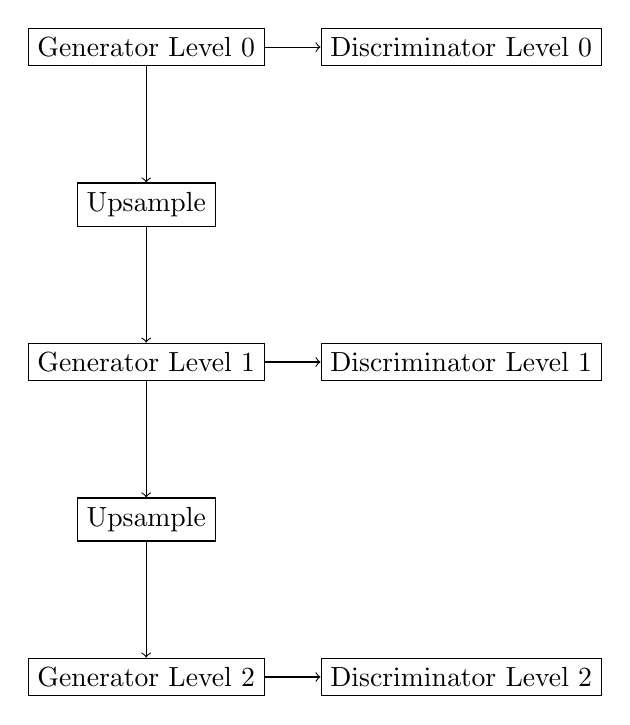
\begin{tikzpicture}[node distance=2cm, auto]
    % Nodes
    \node [draw, rectangle] (G0) {Generator Level 0};
    \node [draw, rectangle, right of=G0, node distance=4cm] (D0) {Discriminator Level 0};
    \node [draw, rectangle, below of=G0] (Upsample0) {Upsample};
    \node [draw, rectangle, below of=Upsample0] (G1) {Generator Level 1};
    \node [draw, rectangle, right of=G1, node distance=4cm] (D1) {Discriminator Level 1};
    \node [draw, rectangle, below of=G1] (Upsample1) {Upsample};
    \node [draw, rectangle, below of=Upsample1] (G2) {Generator Level 2};
    \node [draw, rectangle, right of=G2, node distance=4cm] (D2) {Discriminator Level 2};
    
    % Arrows
    \draw [->] (G0) -- (D0);
    \draw [->] (G0) -- (Upsample0);
    \draw [->] (Upsample0) -- (G1);
    \draw [->] (G1) -- (D1);
    \draw [->] (G1) -- (Upsample1);
    \draw [->] (Upsample1) -- (G2);
    \draw [->] (G2) -- (D2);
\end{tikzpicture}
\end{center}

This diagram illustrates how each generator builds upon the output of the previous level, progressively refining the image.

\subsection{Conclusion}

LAPGAN introduces a novel approach to image generation by leveraging the concept of Laplacian Pyramids~\cite{denton2015deep}. By generating images hierarchically, it effectively captures both global structures and fine details, leading to high-quality high-resolution images~\cite{lai2018fast}. For beginners, implementing LAPGAN provides valuable insights into advanced GAN architectures and techniques for improving image generation.
